% BEAMER ----
% This is just here so I know exactly what I'm looking at in Rstudio when messing with stuff.
\documentclass[10pt,ignorenonframetext,,aspectratio=149]{beamer}
\setbeamertemplate{caption}[numbered]
\setbeamertemplate{caption label separator}{: }
\setbeamercolor{caption name}{fg=normal text.fg}
\usepackage{lmodern}
\usepackage{amssymb,amsmath}
\usepackage{ifxetex,ifluatex}
\usepackage{fixltx2e} % provides \textsubscript
\ifnum 0\ifxetex 1\fi\ifluatex 1\fi=0 % if pdftex
  \usepackage[T1]{fontenc}
  \usepackage[utf8]{inputenc}
\else % if luatex or xelatex
  \ifxetex
    \usepackage{mathspec}
  \else
    \usepackage{fontspec}
  \fi
  \defaultfontfeatures{Ligatures=TeX,Scale=MatchLowercase}
  \newcommand{\euro}{€}
\fi
% use upquote if available, for straight quotes in verbatim environments
\IfFileExists{upquote.sty}{\usepackage{upquote}}{}
% use microtype if available
\IfFileExists{microtype.sty}{%
\usepackage{microtype}
\UseMicrotypeSet[protrusion]{basicmath} % disable protrusion for tt fonts
}{}
\usepackage{natbib}
\bibliographystyle{apsr}
\usepackage{graphicx,grffile}
\makeatletter
\def\maxwidth{\ifdim\Gin@nat@width>\linewidth\linewidth\else\Gin@nat@width\fi}
\def\maxheight{\ifdim\Gin@nat@height>\textheight0.8\textheight\else\Gin@nat@height\fi}
\makeatother
% Scale images if necessary, so that they will not overflow the page
% margins by default, and it is still possible to overwrite the defaults
% using explicit options in \includegraphics[width, height, ...]{}
\setkeys{Gin}{width=\maxwidth,height=\maxheight,keepaspectratio}

% Comment these out if you don't want a slide with just the
% part/section/subsection/subsubsection title:
\AtBeginPart{
  \let\insertpartnumber\relax
  \let\partname\relax
  \frame{\partpage}
}
\AtBeginSection{
  \let\insertsectionnumber\relax
  \let\sectionname\relax
  \frame{\sectionpage}
}
\AtBeginSubsection{
  \let\insertsubsectionnumber\relax
  \let\subsectionname\relax
  \frame{\subsectionpage}
}

\setlength{\emergencystretch}{3em}  % prevent overfull lines
\providecommand{\tightlist}{%
  \setlength{\itemsep}{0pt}\setlength{\parskip}{0pt}}
\setcounter{secnumdepth}{5}

\title{Trimming the Mean of Data with Long Right Tails: The
Bias-Variance Tradeoff}
\author{Xiaoya Wang, Bertrand Sodjahin, and Gradon Nicholls}
\date{}


%% Here's everything I added.
%%--------------------------

\usepackage{graphicx}
\usepackage{rotating}
%\setbeamertemplate{caption}[numbered]
\usepackage{hyperref}
\usepackage{caption}
\usepackage[normalem]{ulem}
%\mode<presentation>
\usepackage{wasysym}
%\usepackage{amsmath}


% Get rid of navigation symbols.
%-------------------------------
\setbeamertemplate{navigation symbols}{}

% Optional institute tags and titlegraphic.
% Do feel free to change the titlegraphic if you don't want it as a Markdown field.
%----------------------------------------------------------------------------------
\institute{June 19, 2023}

% \titlegraphic{\includegraphics[width=0.3\paperwidth]{\string~/Dropbox/teaching/clemson-academic.png}} % <-- if you want to know what this looks like without it as a Markdown field.
% -----------------------------------------------------------------------------------------------------



% Some additional title page adjustments.
%----------------------------------------
\setbeamertemplate{title page}[empty]
%\date{}
\setbeamerfont{subtitle}{size=\small}

\setbeamercovered{transparent}

% Some optional colors. Change or add as you see fit.
%---------------------------------------------------
\definecolor{clemsonpurple}{HTML}{522D80}
 \definecolor{clemsonorange}{HTML}{F66733}
\definecolor{uiucblue}{HTML}{003C7D}
\definecolor{uiucorange}{HTML}{F47F24}

% new gig just dropped
\definecolor{sublue}{HTML}{002F5F}
\definecolor{susky}{HTML}{ACDEE6}
\definecolor{suwater}{HTML}{9BB2CE}





% Some optional color adjustments to Beamer. Change as you see fit.
%------------------------------------------------------------------
\setbeamercolor{frametitle}{fg=sublue,bg=white}
\setbeamercolor{title}{fg=sublue,,bg=white}
\setbeamercolor{local structure}{fg=sublue,}
\setbeamercolor{section in toc}{fg=sublue,bg=white}
% \setbeamercolor{subsection in toc}{fg=clemsonorange,bg=white}
\setbeamercolor{footline}{fg=sublue!50, bg=white}
\setbeamercolor{block title}{fg=sublue,bg=white}
\setbeamercolor{background canvas}{bg=white}


\setbeamercolor{title separator}{fg=suwater}

\let\Tiny=\tiny


% Sections and subsections should not get their own damn slide.
%--------------------------------------------------------------
\AtBeginPart{}
\AtBeginSection{}
\AtBeginSubsection{}
\AtBeginSubsubsection{}

% Suppress some of Markdown's weird default vertical spacing.
%------------------------------------------------------------
\setlength{\emergencystretch}{0em}  % prevent overfull lines
\setlength{\parskip}{0pt}


% Allow for those simple two-tone footlines I like.
% Edit the colors as you see fit.
%--------------------------------------------------
\defbeamertemplate*{footline}{my footline}{%
    \ifnum\insertpagenumber=1
    \hbox{%
        \begin{beamercolorbox}[wd=\paperwidth,ht=.8ex,dp=1ex,center]{}%
      % empty environment to raise height
        \end{beamercolorbox}%
    }%
    \vskip0pt%
    \else%
        \raisebox{0.15cm}[0pt][0pt]{%
         \footnotesize{%
            \begin{minipage}{\textwidth}
               \hspace*{0.1cm} \insertsection \hfill \insertframenumber/\inserttotalframenumber \hspace*{0.1cm}
            \end{minipage}
            }}
        \newline
        \Tiny{%
            \color{sublue}{\rule{\paperwidth}{0.4mm}}\newline%
            \color{suwater}{\rule{\paperwidth}{.4mm}}%
        }%
    \fi%
}

% Various cosmetic things, though I must confess I forget what exactly these do and why I included them.
%-------------------------------------------------------------------------------------------------------
\setbeamercolor{structure}{fg=blue}
\setbeamercolor{local structure}{parent=structure}
\setbeamercolor{item projected}{parent=item,use=item,fg=sublue,bg=white}
\setbeamercolor{enumerate item}{parent=item}

% Adjust some item elements. More cosmetic things.
%-------------------------------------------------
\setbeamertemplate{itemize item}{\color{sublue}$\bullet$}
\setbeamertemplate{itemize subitem}{\color{sublue}\scriptsize{$\bullet$}}
\setbeamertemplate{itemize/enumerate body end}{\vspace{.6\baselineskip}} % So I'm less inclined to use \medskip and \bigskip in Markdown.

% Automatically center images
% ---------------------------
% Note: this is for ![](image.png) images
% Use "fig.align = "center" for R chunks

\usepackage{etoolbox}

\AtBeginDocument{%
  \letcs\oig{@orig\string\includegraphics}%
  \renewcommand<>\includegraphics[2][]{%
    \only#3{%
      {\centering\oig[{#1}]{#2}\par}%
    }%
  }%
}

% I think I've moved to xelatex now. Here's some stuff for that.
% --------------------------------------------------------------
% I could customize/generalize this more but the truth is it works for my circumstances.

\ifxetex


% Commented out -----
%\setbeamerfont{title}{family=\fontspec{\sfdefault}}
%\setbeamerfont{frametitle}{family=\fontspec{\sfdefault}}
\usepackage[font=small,skip=0pt]{caption}
 \else
 \fi

% {modelsummary} and {kableExtra} support
% --------------------------------------------------------------
% Rather than clutter my preambles for this stuff, it's just going to come by default.
\usepackage{dcolumn}
\usepackage{booktabs}
\usepackage{longtable}
\usepackage{array}
\usepackage{multirow}
\usepackage{wrapfig}
\usepackage{float}
\usepackage{colortbl}
\usepackage{pdflscape}
\usepackage{tabu}
\usepackage{threeparttable}


% Some random stuff now...
% ------------------------

\usepackage{tikz}

\newcommand{\shrug}[1][]{%
\begin{tikzpicture}[baseline,x=0.8\ht\strutbox,y=0.8\ht\strutbox,line width=0.125ex,#1]
\def\arm{(-2.5,0.95) to (-2,0.95) (-1.9,1) to (-1.5,0) (-1.35,0) to (-0.8,0)};
\draw \arm;
\draw[xscale=-1] \arm;
\def\headpart{(0.6,0) arc[start angle=-40, end angle=40,x radius=0.6,y radius=0.8]};
\draw \headpart;
\draw[xscale=-1] \headpart;
\def\eye{(-0.075,0.15) .. controls (0.02,0) .. (0.075,-0.15)};
\draw[shift={(-0.3,0.8)}] \eye;
\draw[shift={(0,0.85)}] \eye;
% draw mouth
\draw (-0.1,0.2) to [out=15,in=-100] (0.4,0.95);
\end{tikzpicture}}


% some math packages
\usepackage{accents} % make sure comes AFTER amsmath
\usepackage{bm} % bold math characters
\usepackage{centernot} % add "not" slash to any symbol e.g. \centernot\implies
\usepackage{mathtools}
\usepackage{scalerel}
\usepackage{xintexpr}

% fancy/different versions of letters
\newcommand{\A}{\mathcal{A}} % fancy A
\newcommand{\B}{\mathcal{B}} % fancy B
\newcommand{\F}{\mathcal{F}} % fancy F
\newcommand{\G}{\mathcal{G}} % fancy G
\renewcommand{\L}{\mathcal{L}} % fancy L
\newcommand{\M}{\mathcal{M}} % fancy M
\newcommand{\N}{\mathbb{N}} % natural numbers
\newcommand{\R}{\mathbb{R}} % real numbers
\newcommand{\Z}{\mathbb{Z}} % integers
\renewcommand{\epsilon}{\varepsilon} % use fancy epsilon by default
\newcommand{\eps}{\epsilon} % alias for epsilon

% scalable \hat
\newcommand{\scalehat}[2]{\hstretch{#1}{\hat{\hstretch{\xintieval[7]{1/#1}}{#2}}}}

%%% shortcuts for operators/symbols/relations/etc. %%%
  % operators: probability, expectation, variance, covariance
  \DeclareMathOperator{\PROp}{\textbf{P}} % Probability function --> use "\PR{}"
  \DeclarePairedDelimiterX{\PRArg}[1]{(}{)}{#1}
  \newcommand{\PR}{\PROp\PRArg*}

  \DeclareMathOperator{\EOp}{\mathbb{E}} % Expected Value --> use "\E{}"
  \DeclarePairedDelimiterX{\EArg}[1]{[}{]}{#1}
  \newcommand{\E}{\EOp\EArg*}

  \DeclareMathOperator{\VarOp}{Var} % Variance --> use "\Var{}"
  \DeclarePairedDelimiterX{\VarArg}[1]{(}{)}{#1}
  \newcommand{\Var}{\VarOp\VarArg*}
  \newcommand{\hatVar}{\scalehat{2}{\VarOp}\VarArg*}

  \DeclareMathOperator{\CovOp}{Cov} % Covariance --> use "\Cov{}"
  \DeclarePairedDelimiterX{\CovArg}[1]{(}{)}{#1}
  \newcommand{\Cov}{\CovOp\CovArg*}

  \DeclareMathOperator{\CorrOp}{Corr} % Correlation --> use "\Corr{}"
  \DeclarePairedDelimiterX{\CorrArg}[1]{(}{)}{#1}
  \newcommand{\Corr}{\CorrOp\CorrArg*}

  % some probability stuff
  \newcommand{\indfun}{\textbf{1}} % indicator function
  \newcommand{\indep}{\perp \!\!\! \perp} % independence symbol between r.v.s
  \newcommand{\eqdist}{\overset{\text{d}}{=}} % denotes two r.v. are equal in distn
  \newcommand{\chf}{\varphi} % characteristic function
  \newcommand{\distas}[2]{\sim \text{{#1}} \left({#2}\right)} % random variable distributed as
  \newcommand{\iidas}[2]{\overset{\text{iid}}{\sim} \text{{#1}} \left({#2}\right)} % iid rv's distributed as
  \newcommand{\indepas}[2]{\overset{\text{ind.}}{\sim} \text{{#1}} \left({#2}\right)} % independent rv's distributed as
  \newcommand{\approxas}[2]{\overset{\cdot}{\sim} \text{{#1}} \left({#2}\right)} % rv's approximately distributed as
  \newcommand{\suchthat}{\,\, | \,\,} % --> vertical line for conditioning
  \newcommand{\pto}{\overset{\text{p}}{\to}} % converge in probability
  \newcommand{\asto}{\overset{\text{a.s.}}{\to}} % converge almost surely
  \newcommand{\dto}{\overset{\text{d}}{\to}} % converge in distribution
  \newcommand{\Lpto}[1]{\overset{\L^{#1}}{\to}} % Lp convergence

  % some mathy stuff
  \newcommand{\notimply}{\centernot\implies} % does not imply
  \newcommand{\notimplies}{\notimply} % alias for notimply
  \let\bforall\forall % forall at beginning of expression
  \renewcommand{\forall}{\,\,\,\bforall} % forall in middle of expression (added hspace)
  \newcommand{\transpose}{\intercal} % transpose T
  \newcommand{\vect}[1]{\underaccent{\bar}{#1}} % vector shown as undebar
  \newcommand{\floor}[1]{\left\lfloor{#1}\right\rfloor} % floor function
  \newcommand{\ceil}[1]{\left\lceil{#1}\right\rceil} % celing function
  \renewcommand{\th}{^{\text{th}}} % convenience to write, e.g., n^th, i^th, etc.

%%%%%%%%%%%%%%%%%%%%%%%%%%%%%%%%%%%%%%%%%%%%%%%%%%%%%%%%%%



% header includes go last.


% Okay, and begin the actual document...

\begin{document}
\frame{\addtocounter{framenumber}{-1}
\titlepage}





\hypertarget{motivation}{%
\section{Motivation}\label{motivation}}

\begin{frame}{Motivation}
\protect\hypertarget{motivation-1}{}
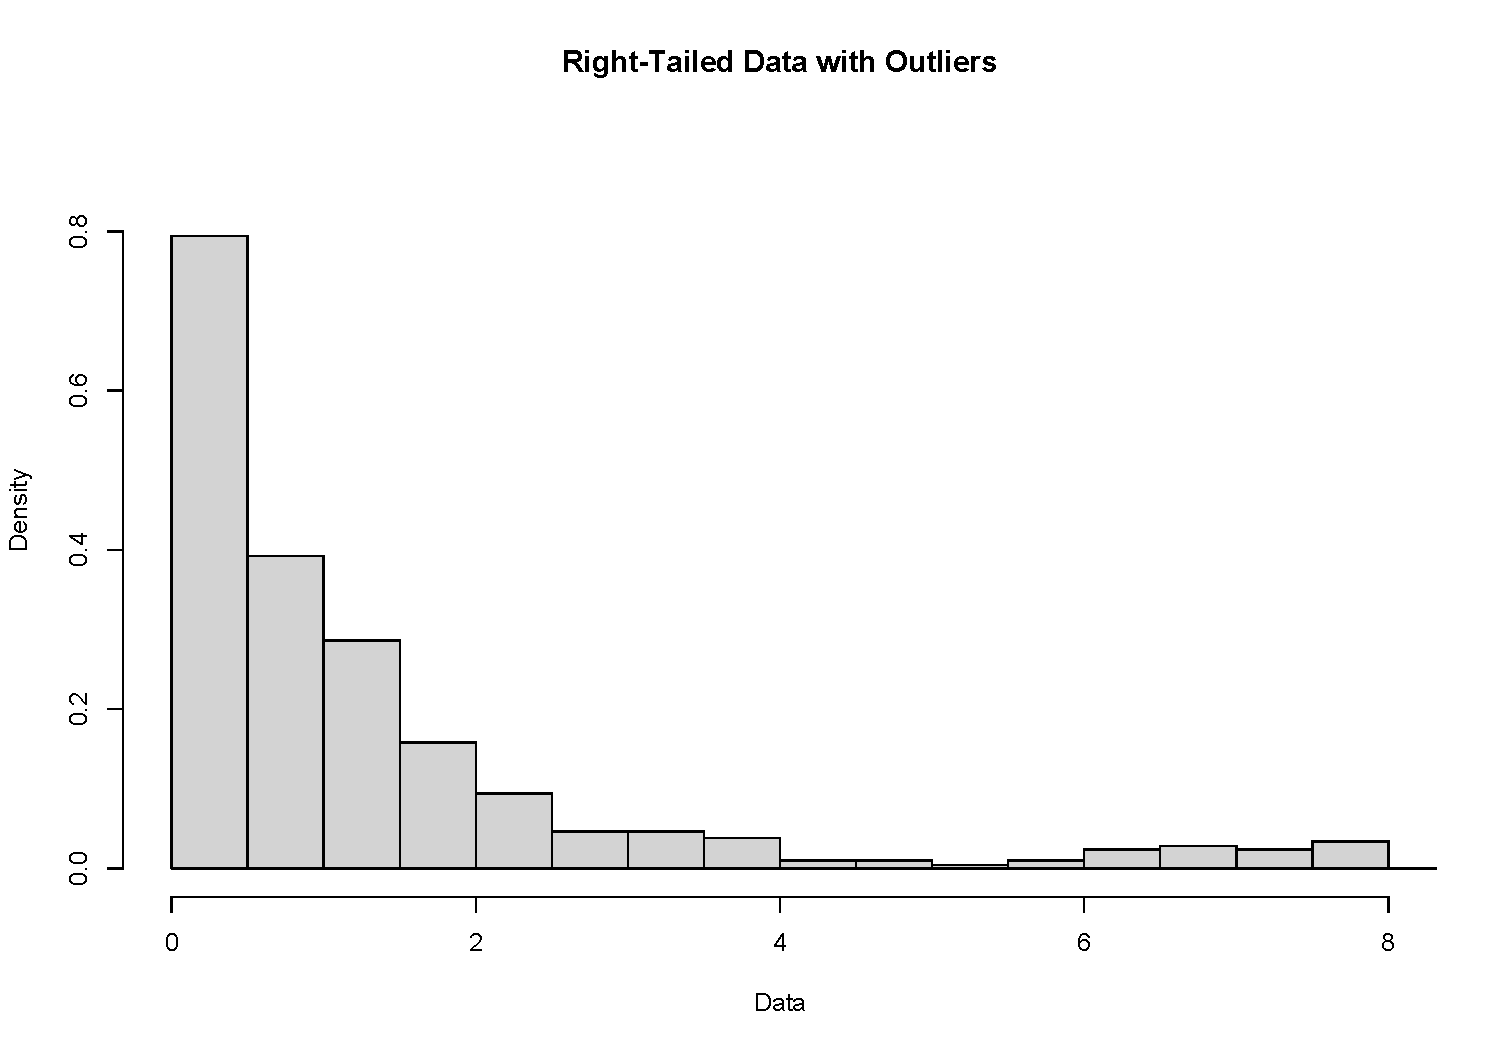
\includegraphics[height=0.6\textheight]{figs/unnamed-chunk-1}

\begin{itemize}
\tightlist
\item
  Goal: Compute sample average.
\item
  Challenge: Are outliers ``true'' outliers or not?
\item
  Even if true outliers, sample average may have large variance.
\end{itemize}
\end{frame}

\begin{frame}{Trimming the Mean}
\protect\hypertarget{trimming-the-mean}{}
Let \(Y_i \iidas{F}{\cdot}\). The sample mean is

\[
\hat\mu_0 = \frac{\sum\limits_{i=1}^n Y_i}{n}.
\]

To reduce the influence of outliers in the right tail, could use trimmed
mean: remove the top \(100p\%\) of observations:

\[
\hat\mu_p = \frac{\sum\limits_{i=1}^n I(Y_i \leq Y_{(1-p)}) Y_i }{\sum\limits_{i=1}^n I(Y_i \leq Y_{(1-p)})}
\]

where \(Y_{(1-p)}\) is the \(1-p\th\) quantile from the sample data.
\end{frame}

\begin{frame}{Example: 5\% Trimming}
\protect\hypertarget{example-5-trimming}{}
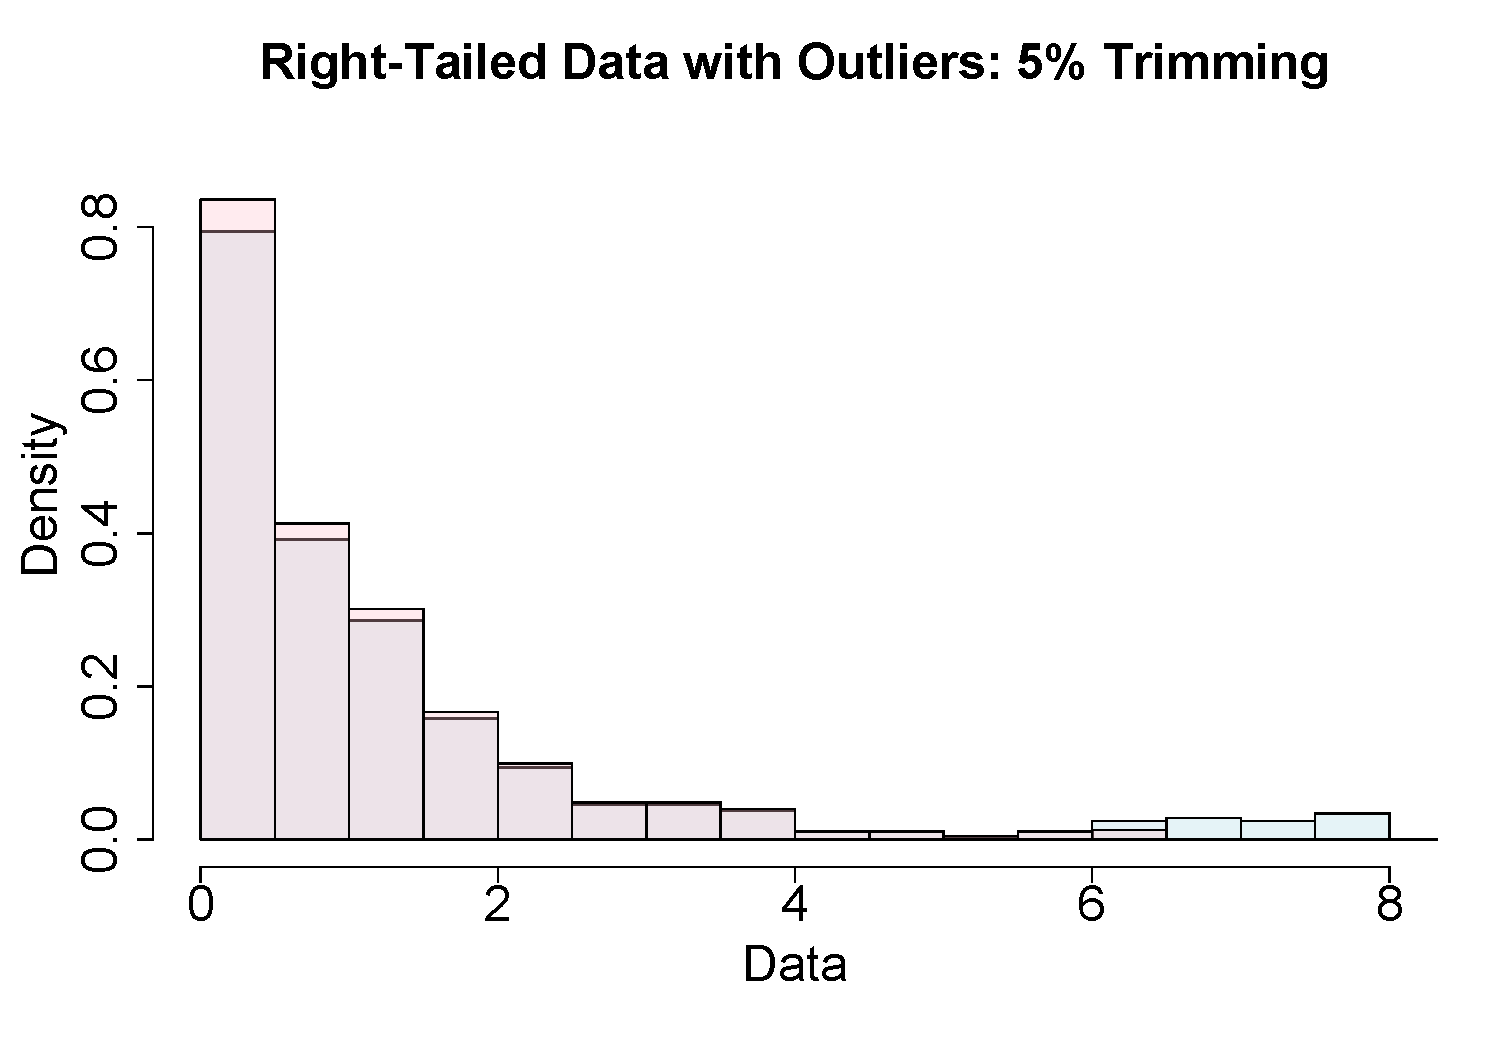
\includegraphics{figs/unnamed-chunk-2.pdf}
\end{frame}

\begin{frame}{Bias-Variance Tradeoff}
\protect\hypertarget{bias-variance-tradeoff}{}
\begin{itemize}
\tightlist
\item
  Is there any value to trimming if there are no ``true'' outliers?
\item
  Trimming reduces large values \(\to\) decrease in variance, increase
  in bias.
\item
  Overall, may observe reduction in MSE:
\end{itemize}

\[
\text{MSE} = \text{Bias}^2 + \text{Variance}
\]

\textbf{Research Question:} How does trimming affect bias, variance, MSE
of estimator if there are no outliers?

\textbf{Assumption:} We assume underlying data generated from a Weibull
random variable.
\end{frame}

\hypertarget{weibull}{%
\section{Weibull}\label{weibull}}

\begin{frame}{The Weibull Distribution
\small e.g.~\cite{bain1992introduction}}
\protect\hypertarget{the-weibull-distribution-e.g.}{}
\(X \distas{Wei}{\theta,\beta}\):

\[
f(x; \,\theta, \beta) = \frac{\beta}{\theta} \left(\frac{x}{\theta}\right)^{\beta-1} e^{-(x / \theta)^\beta}
\]

\begin{itemize}
\tightlist
\item
  \(\theta\): scale
  parameter--i.e.~\(X \distas{Wei}{\theta, \beta} \implies \frac{X}{\theta} \distas{Wei}{1,\beta}\)

  \begin{itemize}
  \tightlist
  \item
    Interested in relative efficiency--WLOG assume \(\theta = 1\)
  \end{itemize}
\item
  \(\beta\): shape parameter

  \begin{itemize}
  \tightlist
  \item
    \(\beta = 1\): exponential distribution
  \item
    \(\beta > 1\): polynomial times exponential
  \item
    \(\beta < 1\): inverse polynomial times exponential -- asymptote at
    0
  \end{itemize}
\end{itemize}

\[
\E{X} = \theta \Gamma(1 + 1/\beta)
\]

\[
\Var{X} = \theta^2 \left( \Gamma(1 + 2/\beta) - \Gamma^2(1 + 1/\beta) \right)
\]
\end{frame}

\begin{frame}{Shape of the Weibull}
\protect\hypertarget{shape-of-the-weibull}{}
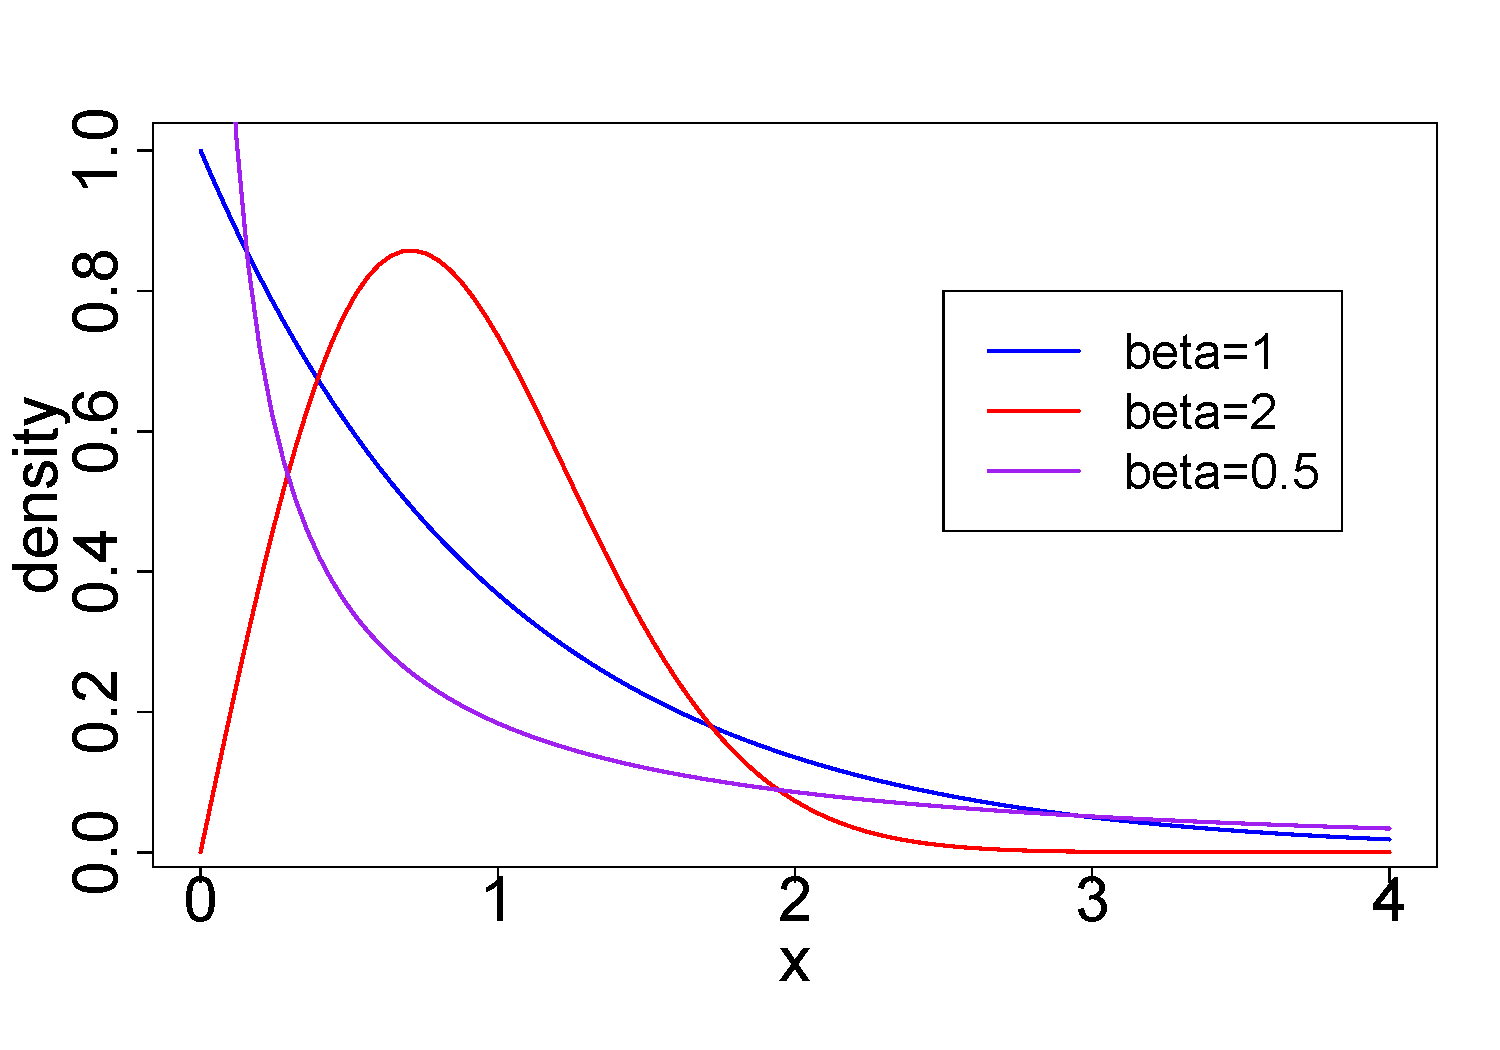
\includegraphics[height=0.7\textheight]{figs/unnamed-chunk-3}

We will consider only values \(\beta \in (0,1)\).
\end{frame}

\begin{frame}{Maximum Likelihood Estimation of the Mean}
\protect\hypertarget{maximum-likelihood-estimation-of-the-mean}{}
\begin{itemize}
\setlength\itemsep{0.5cm}
\item Assume $Y_i \iidas{Wei}{\theta,\beta}$. Let $\mu = \E{Y_i} = \theta\Gamma(1 + 1/\beta)$.
\item $\hat\mu_{\text{MLE}} = \hat\theta_{\text{MLE}} \Gamma(1 + 1 / \hat\beta_{\text{MLE}})$ by invariance property.
\item $\hat\theta_{\text{MLE}},\hat\beta_{\text{MLE}}$ have no closed form, rely on numerical methods
\item For large $n$, $\Var{\hat\mu_\text{MLE}}$ achieves Cramer-Rao lower bound, and so can be used as "gold standard" baseline.
\item For small $n$, less certain.
\end{itemize}
\end{frame}

\hypertarget{simulation}{%
\section{Simulation}\label{simulation}}

\begin{frame}{Simulation}
\protect\hypertarget{simulation-1}{}
Parameters:

\begin{itemize}
\tightlist
\item
  \(\beta \in (0,1)\)
\item
  \(n \in \{20,200,2000\}\)
\item
  \(p \in \{0.01, 0.025, 0.05, 0.1\}\)
\end{itemize}

Simulation:

\begin{itemize}
\tightlist
\item
  for \(s = 1,\dots,S\)

  \begin{itemize}
  \tightlist
  \item
    gen \(Y_i^s \iidas{Wei}{1,\beta}\), \(i = 1, \cdots, n\)
  \item
    estimate \(\hat\mu_0^s\), \(\hat\mu_p^s\),
    \(\hat\mu_{\text{MLE}}^s\)
  \end{itemize}
\end{itemize}

Estimate:

\begin{itemize}
\tightlist
\item
  Bias: \(\frac{\sum_s \hat\mu^s}{S} - \Gamma(1 + 1/\beta)\)
\item
  Variance:
  \(\frac{\sum_s \left(\hat\mu^s - (1/n)\sum_s \hat\mu^s\right)^2}{S-1}\)
\item
  MSE: \(\text{Bias}^2 + \text{Var}\)
\end{itemize}
\end{frame}

\begin{frame}{(Preliminary?) Results}
\protect\hypertarget{preliminary-results}{}
\begin{itemize}
\tightlist
\item
  \ldots\ldots{}
\end{itemize}
\end{frame}

\begin{frame}{Conclusions}
\protect\hypertarget{conclusions}{}
\begin{itemize}
\tightlist
\item
  \ldots\ldots{}
\end{itemize}
\end{frame}

\begin{frame}[allowframebreaks]{}
\bibliography{bib.bib}
\end{frame}


\end{document}
